\documentclass{article}
\usepackage[utf8]{inputenc}
\usepackage[margin = 1.1in, headheight = 0.9in, footskip = 0.75 in]{geometry}
\usepackage{fancyhdr}
\usepackage{lastpage}
\usepackage{amsmath}
\usepackage{amssymb}
\usepackage{xparse}
\usepackage{graphicx}
\usepackage{enumerate}
\usepackage{mathtools}
\usepackage{amsthm}
\usepackage{tikz-cd}
\usepackage{tikz}
\usepackage{array}
\usepackage{pgfplots}
\usepackage{bbm}
\usepackage[shortlabels]{enumitem}
\usepackage{algorithm}
\usepackage{algpseudocode}
\usepackage{booktabs}
\usepackage{hyperref}
\hypersetup{
    colorlinks=true,
    linkcolor=black,
    filecolor=magenta,      
    urlcolor=red
    }

\urlstyle{same}
\newcommand{\RNum}[1]{\uppercase\expandafter{\romannumeral #1\relax}}
\newcommand\ddfrac[2]{\frac{\displaystyle #1}{\displaystyle #2}}
\usepackage{xpatch}
\setlength{\parindent}{3em}
\setlength{\parskip}{0.5em}
\newcolumntype{C}{>{\centering\arraybackslash}p{1cm}}
%===================================================================================================
\pagestyle{fancyplain}
\renewcommand{\headrulewidth}{0pt}
\renewcommand{\footrulewidth}{0pt}
\fancyhf{}\par 
\lhead{\hspace{0cm}\\\hspace{0cm}\\Zmh6339\\AI \& Machine Learning, CS-UH 3260\\Professor Keith Ross}
\rhead{Ziad Hassan\\ February 12, 2024}
\cfoot{\thepage/\pageref{LastPage}}
%===================================================================================================
\title{Assignment 2}
\date{}
\author{}
%===================================================================================================
\begin{document}
\maketitle
%==================================================================================================
\section*{Question 1}
Below is the plotting of $Q(\texttt{s,stick})$\\ 
where $s\coloneq(\texttt{player total} = 18, \texttt{dealer showing} = 8, \texttt{no usable ace})$
in the first MCES version of the Blackjack game over 10,000 training epsiodes (where every 100th episode was recorded).
\begin{center}
    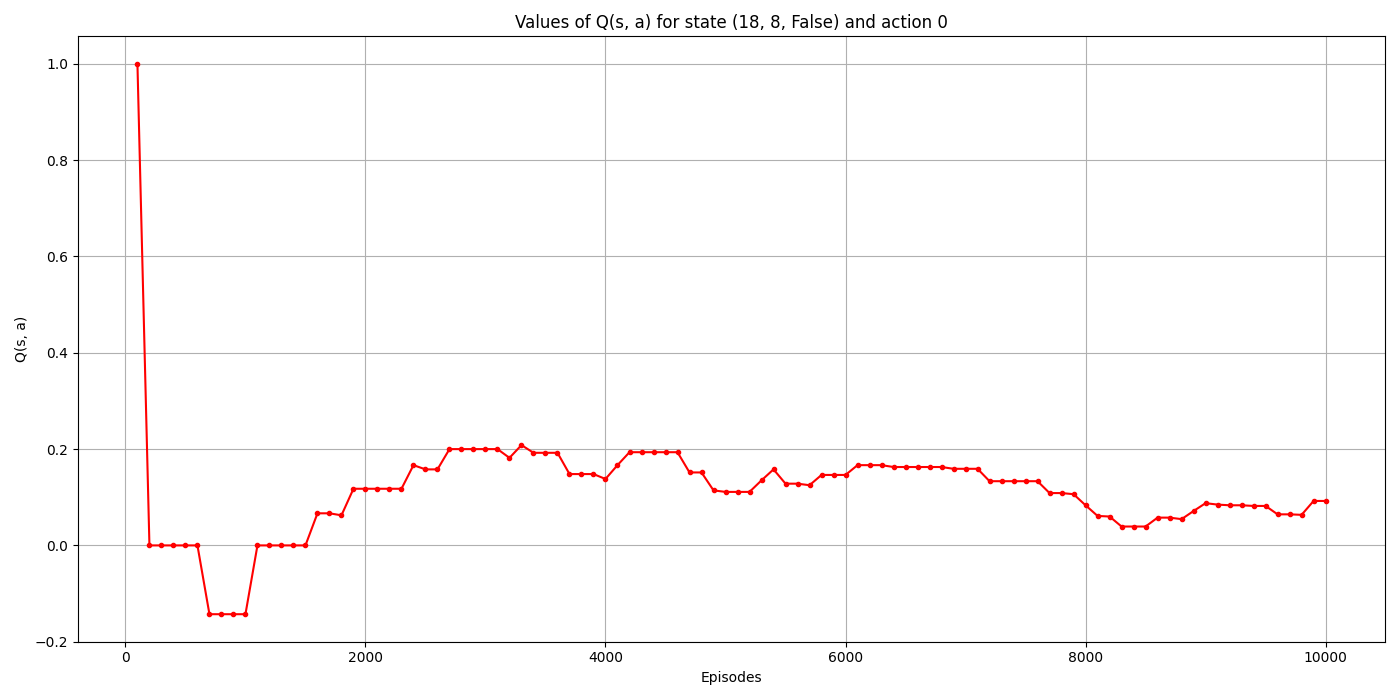
\includegraphics[scale=0.4]{Q_values.png}
\end{center}\par 
Moreover, here are the winning, drawing, and losing rates of the first MCES version of the Blackjack game after 10,000 training episodes and then 100,000 testing episodes.
\begin{center}
    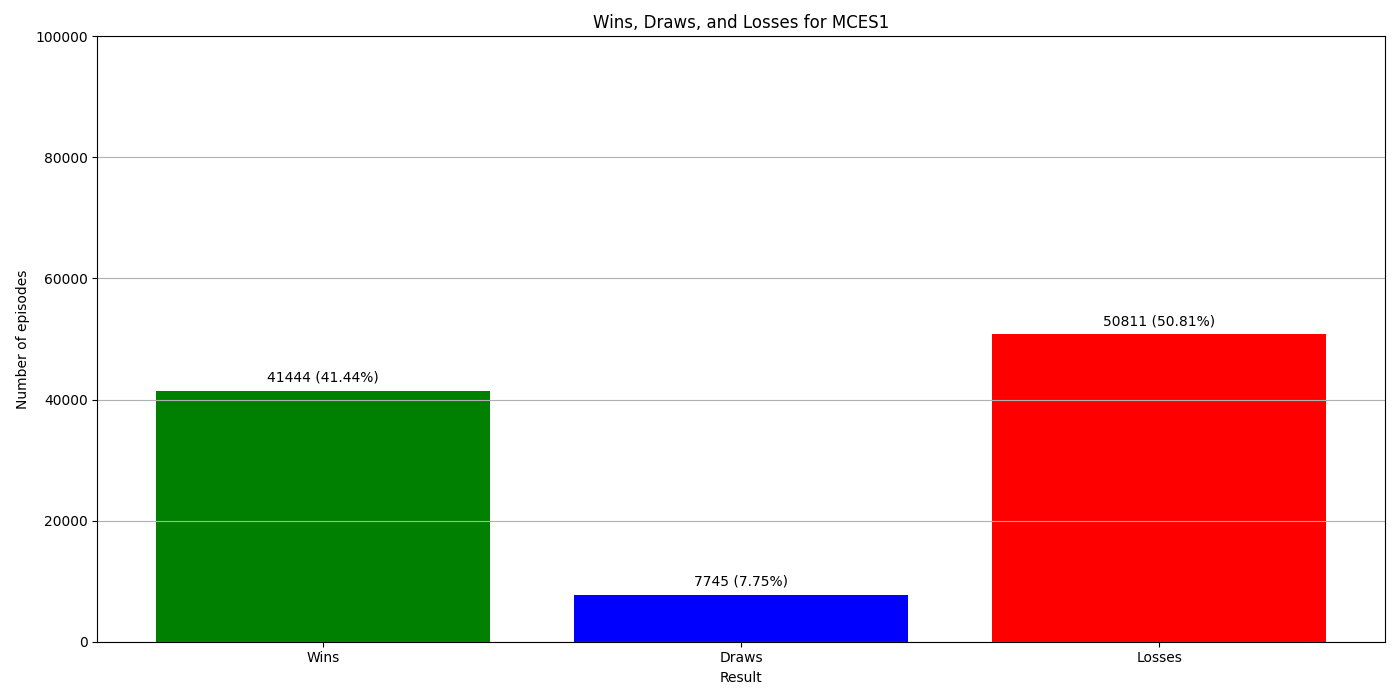
\includegraphics[scale=0.4]{MCES1_Wins_Draws_Losses.png}
\end{center}
%==================================================================================================
\section*{Question 2}
Below is the plotting of $Q(\texttt{s,stick})$\\ 
where $s\coloneq(\texttt{player total} = 18, \texttt{dealer showing} = 8, \texttt{no usable ace})$
in the second MCES version of the Blackjack game over 10,000 training epsiodes (where every 100th episode was recorded).
\begin{center}
    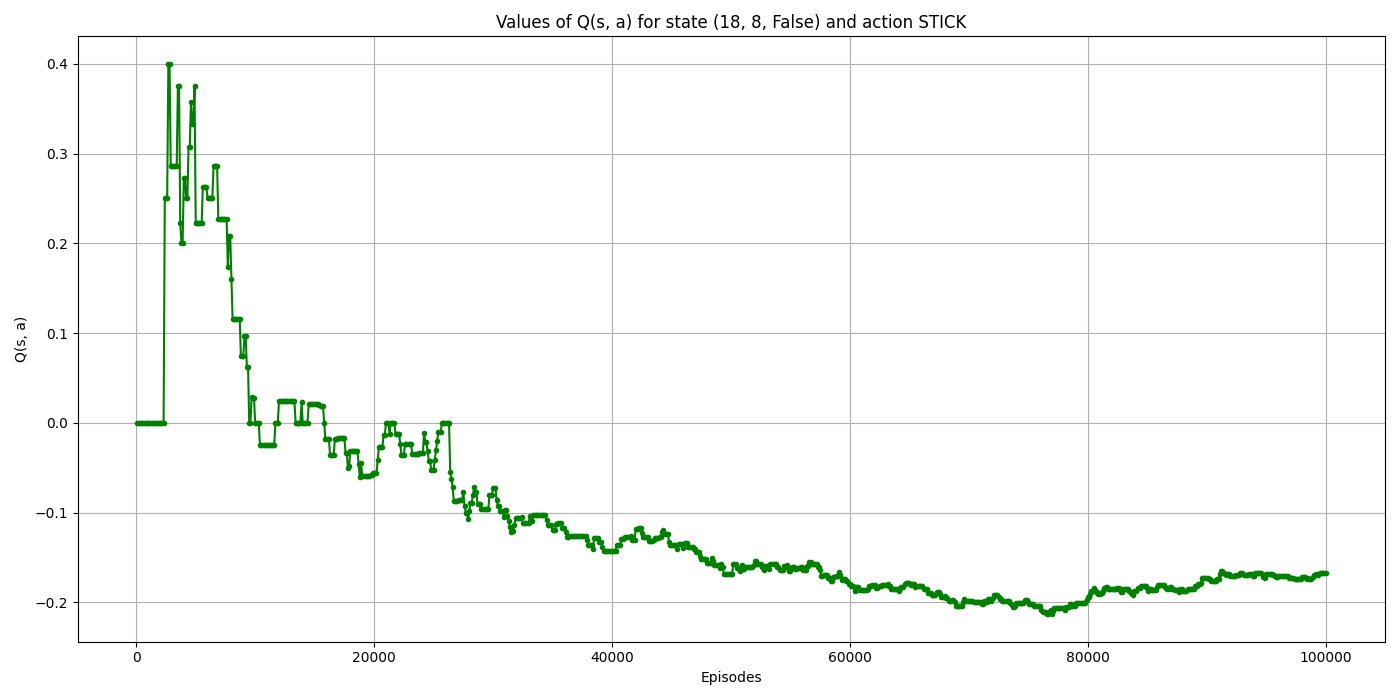
\includegraphics[scale=0.4]{Q_values2.png}
\end{center}\par 
Moreover, here are the winning, drawing, and losing rates of the second MCES version of the Blackjack game after 10,000 training episodes and then 100,000 testing episodes.
\begin{center}
    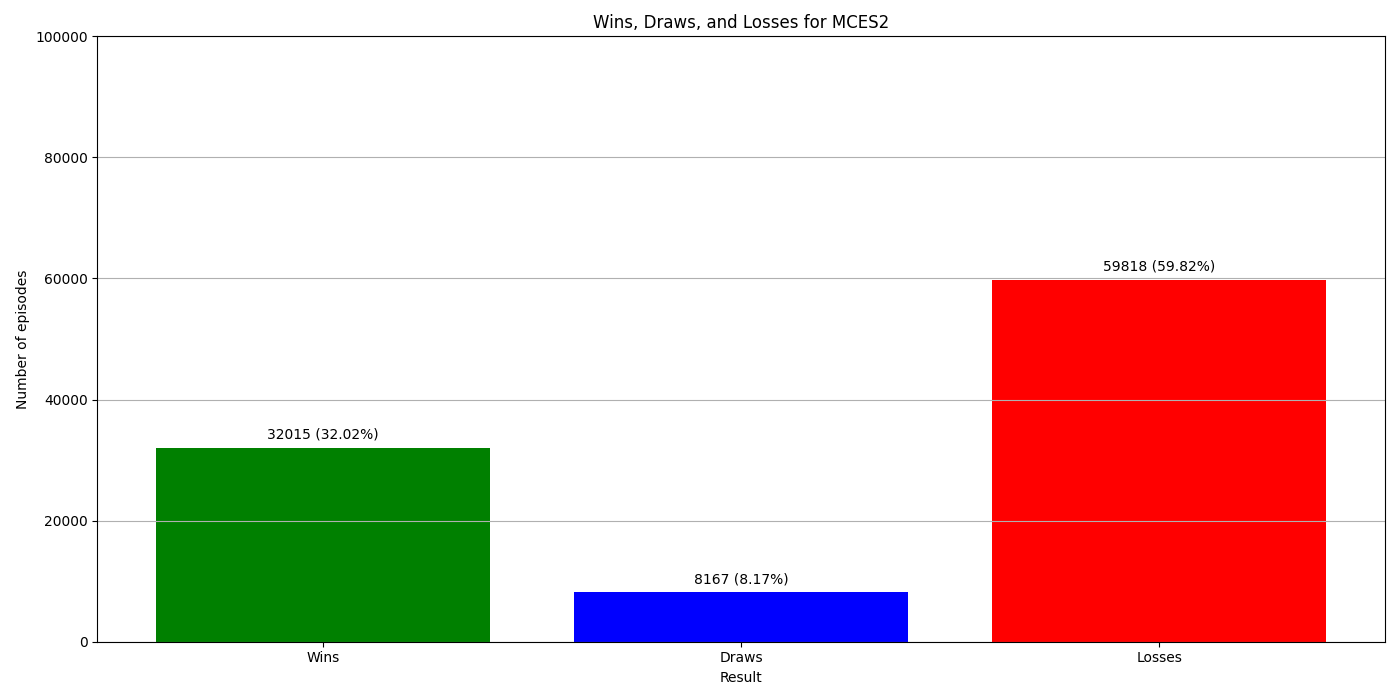
\includegraphics[scale=0.4]{MCES2_Wins_Draws_Losses.png}
\end{center}
%==================================================================================================
\section*{Question 3}
Below is the plotting of $Q(\texttt{s,stick})$\\ 
where $s\coloneq(\texttt{player total} = 18, \texttt{dealer showing} = 8, \texttt{no usable ace})$
in the Q-learning version of the Blackjack game with $\alpha = 0.01$ and $\alpha=0.1$ over all 100,000 training epsiodes.
\begin{center}
    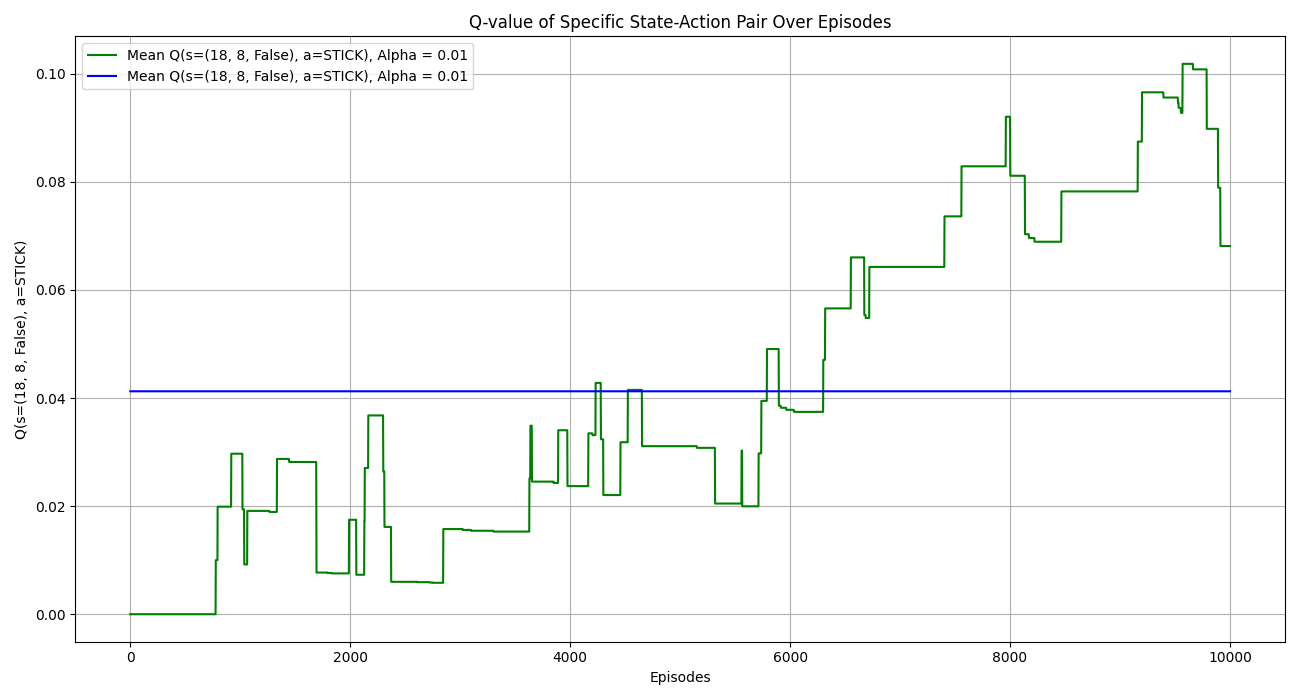
\includegraphics[scale=0.4]{Q_Blackjack_Alpha_0.01.png}
    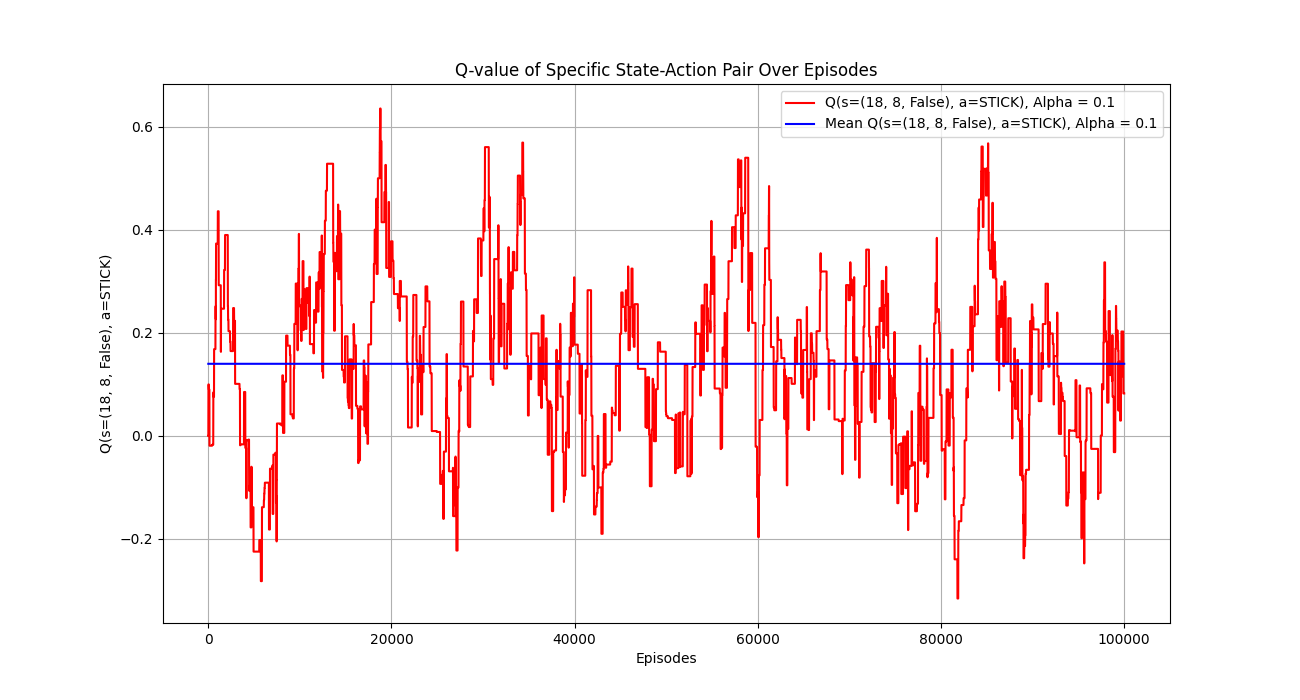
\includegraphics[scale=0.4]{Q_Blackjack_Alpha_0.1.png}
\end{center}\par 
Moreover, here are the winning, drawing, and losing rates of the Q-learning version of the Blackjack game with $\alpha = 0.01$ and $\alpha=0.1$ after 100,000 testing episodes with each 2000th training episode (total of 50 averages).
\begin{center}
    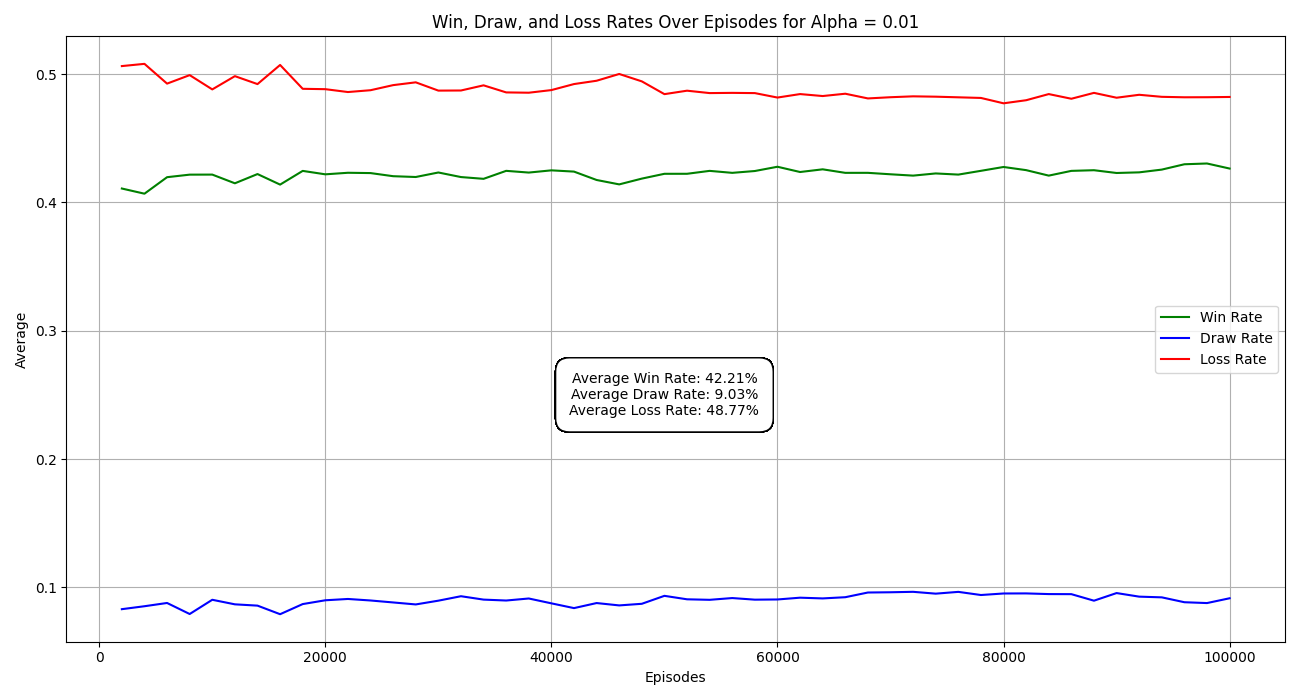
\includegraphics[scale=0.4]{Win_Draw_Loss_Rates_Alpha_0.01.png}
    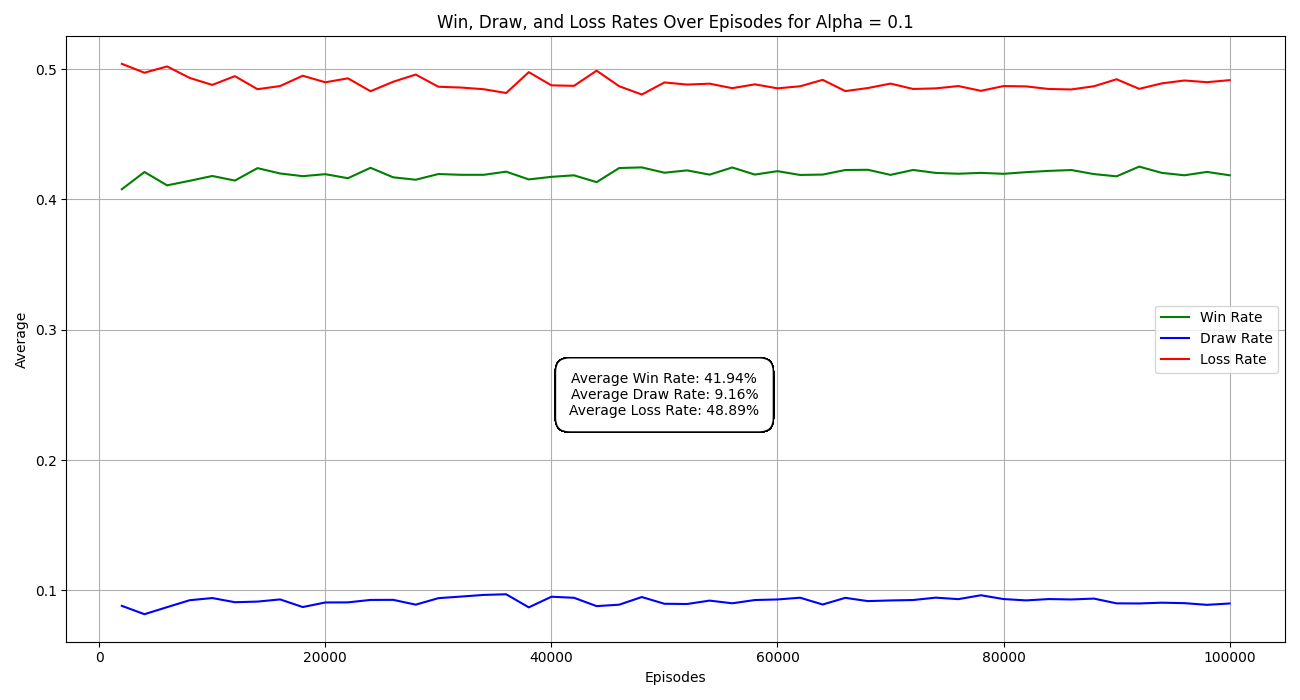
\includegraphics[scale=0.4]{Win_Draw_Loss_Rates_Alpha_0.1.png}
\end{center}\par 

\subsection*{\underline{Differences Between Algorithms}}
The MCES1 plot indicates a win rate of about 41.44\% and a loss rate of 50.81\%. 
The MCES2 plot shows a lower win rate of 32.02\% and a higher loss rate of 59.82\%.
The Q-learning plots for both alpha values (0.1 and 0.01) seem to show an average win rate of approximately 42\%, with a loss rate hovering around 49\%. 
This suggests that Q-learning maintains a more consistent win/loss ratio across different learning rates compared to MCES.
\hfill\\\\
MCES1 has a draw rate of 7.75\%, and MCES2 has a slightly higher draw rate of 8.17\%.
Q-learning has slightly higher draw rates, with 9.16\% for alpha 0.1 and 9.03\% for alpha 0.01. 
This could indicate that the Q-learning policy is slightly more conservative, leading to more ties. 
It may also reflect a better balanced strategy that avoids losses by not taking unnecessary risks, resulting in slightly more draws.
\hfill\\\\
For Q-learning, changing the alpha value from 0.1 to 0.01 does not seem to significantly affect the win and loss rates.
However, it may influence the stability of learning. 
Typically, a smaller alpha would result in smoother learning curves as it integrates new information more conservatively.
This can be slightly observed in the Q-learning plots, where the win and loss rates for alpha 0.01 are slightly more stable than those for alpha 0.1.
\hfill\\\\
The Q-values plots show the value of a specific state-action pair over episodes. For alpha 0.1, the plot exhibits more variance, indicating less stability in the action-value estimates. This is expected as a higher alpha means that new information has a greater impact on the value updates.
For alpha 0.01, the Q-values plot is smoother, suggesting more stability in the learning process due to the smaller alpha value, which integrates new information more slowly.
\hfill\\\\
MCES exhibits a varying win/loss ratio between the two plots, suggesting that the results can differ significantly depending on the specifics of the MCES implementation or the conditions of the simulation.
Q-learning appears to produce more consistent results across different alpha values, with a slight tendency towards more draws, which might suggest a more cautious approach.
The alpha value in Q-learning does not seem to drastically alter the win/draw/loss rates but does affect the stability of the Q-value estimates, with a lower alpha leading to smoother updates.
The slight increase in draw rates for Q-learning could imply a policy that is more risk-averse and better balanced, leading to more ties.
%==================================================================================================
\end{document}
